\documentclass[
    11pt, % The default document font size, options: 10pt, 11pt, 12pt
    %oneside, % Two side (alternating margins) for binding by default, uncomment to switch to one side
    english, % ngerman for German
    singlespacing, % Single line spacing, alternatives: onehalfspacing or doublespacing
    %draft, % Uncomment to enable draft mode (no pictures, no links, overfull hboxes indicated)
    %nolistspacing, % If the document is onehalfspacing or doublespacing, uncomment this to set spacing in lists to single
    %liststotoc, % Uncomment to add the list of figures/tables/etc to the table of contents
    %toctotoc, % Uncomment to add the main table of contents to the table of contents
    %parskip, % Uncomment to add space between paragraphs
    %nohyperref, % Uncomment to not load the hyperref package
    headsepline, % Uncomment to get a line under the header
    chapterinoneline, % Uncomment to place the chapter title next to the number on one line
    %consistentlayout, % Uncomment to change the layout of the declaration, abstract and acknowledgements pages to match the default layout
    ]{MastersDoctoralThesis} % The class file specifying the document structure

%%%%%%%%%%%%%%%%%%%%%%%%%%%%%%%%%%%%%%%%%
% Masters/Doctoral Thesis 
% LaTeX Template
% Version 2.4 (22/11/16)
%
% This template has been downloaded from:
% http://www.LaTeXTemplates.com
%
% Version 2.x major modifications by:
% Vel (vel@latextemplates.com)
%
% This template is based on a template by:
% Steve Gunn (http://users.ecs.soton.ac.uk/srg/softwaretools/document/templates/)
% Sunil Patel (http://www.sunilpatel.co.uk/thesis-template/)
%
% Template license:
% CC BY-NC-SA 3.0 (http://creativecommons.org/licenses/by-nc-sa/3.0/)
%
%%%%%%%%%%%%%%%%%%%%%%%%%%%%%%%%%%%%%%%%%

%----------------------------------------------------------------------------------------
%	PACKAGES AND OTHER DOCUMENT CONFIGURATIONS
%----------------------------------------------------------------------------------------

\documentclass[
    11pt, % The default document font size, options: 10pt, 11pt, 12pt
    %oneside, % Two side (alternating margins) for binding by default, uncomment to switch to one side
    english, % ngerman for German
    singlespacing, % Single line spacing, alternatives: onehalfspacing or doublespacing
    %draft, % Uncomment to enable draft mode (no pictures, no links, overfull hboxes indicated)
    %nolistspacing, % If the document is onehalfspacing or doublespacing, uncomment this to set spacing in lists to single
    %liststotoc, % Uncomment to add the list of figures/tables/etc to the table of contents
    %toctotoc, % Uncomment to add the main table of contents to the table of contents
    %parskip, % Uncomment to add space between paragraphs
    %nohyperref, % Uncomment to not load the hyperref package
    headsepline, % Uncomment to get a line under the header
    %chapterinoneline, % Uncomment to place the chapter title next to the number on one line
    %consistentlayout, % Uncomment to change the layout of the declaration, abstract and acknowledgements pages to match the default layout
    ]{MastersDoctoralThesis} % The class file specifying the document structure
    
\usepackage[utf8]{inputenc} % Required for inputting international characters
\usepackage[T1]{fontenc} % Output font encoding for international characters

\usepackage{palatino} % Use the Palatino font by default

\usepackage[backend=bibtex,style=numeric,giveninits=true,natbib=true,sorting=none]{biblatex} % Use authoryear citation style for "Author, year" citation style

\addbibresource{references.bib} % The filename of the bibliography

%\usepackage{refcheck} % checks for correct reference usage and produces warnings; enable \nocite command

\usepackage[autostyle=true]{csquotes} % Required to generate language-dependent quotes in the bibliography

\usepackage{float} % In order to use the [H] option for figure alignment

\usepackage{fancyvrb} % keep tabs in verbatim sections, see: https://tex.stackexchange.com/questions/231083/how-to-stop-verbatim-from-converting-tabs-to-spaces

\usepackage{listings} % enable to reference source code, see: ttps://tex.stackexchange.com/questions/74155/how-to-treat-verbatim-as-a-block-that-can-be-referenced-just-like-a-figure

\usepackage{amssymb} % The amssymb package provides various useful mathematical symbols

\usepackage{mathtools} % math tools (ceiling signs, see: http://tex.stackexchange.com/questions/42271/floor-and-ceiling-functions)
\DeclarePairedDelimiter{\ceil}{\lceil}{\rceil}

% following packages allows to write algorithms as pseudocode
\usepackage{amsmath}
\usepackage{algorithmicx}
\usepackage{algorithm}
\usepackage{algpseudocode}
\algnewcommand\algorithmicinput{\textbf{INPUT:}}
\algnewcommand\INPUT{\item[\algorithmicinput]}
\algnewcommand\algorithmicoutput{\textbf{OUTPUT:}}
\algnewcommand\OUTPUT{\item[\algorithmicoutput]}

\usepackage{caption}
\captionsetup{width=0.8\textwidth} % global width of captions in figures, tables, etc. https://tex.stackexchange.com/questions/110393/too-wide-figure-caption

%----------------------------------------------------------------------------------------
%	COMMAND DEFINITIONS
%----------------------------------------------------------------------------------------

\definecolor{todoColor}{rgb}{1,0.55,0.2}
\newcommand{\todo}[1]{\textit{\color{todoColor}#1}}

% define commands to keep the formatting separated from the content 
\newcommand{\keyword}[1]{\textbf{#1}}
%\newcommand{\tabhead}[1]{\textbf{#1}}
\newcommand{\code}[1]{\texttt{#1}}
\newcommand{\file}[1]{\texttt{\bfseries#1}}
\newcommand{\option}[1]{\texttt{\itshape#1}}
\newcommand{\tabhead}[1]{\textbf{#1}}
\newcommand*\diff{\mathop{}\!\mathrm{d}} % dx
\newcommand*\Diff[1]{\mathop{}\!\mathrm{d^#1}} % d^2x
\newcommand{\mtrx}[1]{\mathbf{#1}}

%----------------------------------------------------------------------------------------
%	MARGIN SETTINGS
%----------------------------------------------------------------------------------------

\geometry{
    paper=a4paper, % Change to letterpaper for US letter
    inner=2.5cm, % Inner margin
    outer=3.8cm, % Outer margin
    bindingoffset=.5cm, % Binding offset
    top=1.5cm, % Top margin
    bottom=1.5cm, % Bottom margin
    %showframe, % Uncomment to show how the type block is set on the page
}

%----------------------------------------------------------------------------------------
%	THESIS INFORMATION
%----------------------------------------------------------------------------------------
\title{Doctoral Thesis}
\thesistitle[0, 0]{Multimesh Methods for Data Visualization and Finite Element Analysis} % Your thesis title, this is used in the title and abstract, print it elsewhere with ttitle
\thesistitlecs{V\'ices\'i\v{t}ov\'e metody pro vizualizaci dat a v\'ypo\v{c}ty MKP} % Your thesis title in Czech, this is used in the title and abstract, print it elsewhere ith \ttitlecs
\supervisor{prof. Ing. Jaroslav Kruis, Ph.D.} % Your supervisor's name, this is used in the title page, print it elsewhere with \supname
\examiner{} % Your examiner's name, this is not currently used anywhere in the template, print it elsewhere with \examname
\degree{Doctor of Philosophy} % Your degree name, this is used in the title page and abstract, print it elsewhere with \degreename
\author{Ing. \v{S}t\v{e}p\'{a}n Bene\v{s}} % Your name, this is used in the title page, print it elsewhere with \authorname
\authornodegree{\v{S}t\v{e}p\'{a}n Bene\v{s}} % Your name without degrees, this is used in the abstract and declaration page, print it elsewhere with \authornamenodegree
\addresses{Th\'akurova 7, 166 29 Praha 6} % Your address, this is not currently used anywhere in the template, print it elsewhere with \addressname

\subject{Engineering software} % Your subject area, this is not currently used anywhere in the template, print it elsewhere with \subjectname
\keywords{Finite Element Method (FEM), Finite Element Analysis (FEA), Post-processing, Data visualization, Data compression, Data management, Singular Value Decomposition SVD)} % Keywords for your thesis, this is not currently used anywhere in the template, print it elsewhere with \keywordnames
\keywordscs{Metoda kone\v{c}n\'ych prvk\r{u} (MKP), Kone\v{c}n\v{e} prvkov\'a anal\'yza, Vizualizace dat, Komprese dat, Spr\'ava dat, Singul\'arn\'i rozklad (SVD)} % Keywords or your thesis, this is not currently used anywhere in the template, print it elsewhere with \keywordnames
\university{\href{http://www.cvut.cz}{Czech Technical University in Prague}} % Your university's name and URL, this is used in the title page and abstract, print it elsewhere ith \univname
\department{\href{http://mech.fsv.cvut.cz}{Department of Mechanics}} % Your department's name and URL, this is used in the title page and abstract, print it elsewhere with deptname
\faculty{\href{http://www.fsv.cvut.cz}{Faculty of Civil Engineering}} % Your faculty's name and URL, this is used in the title page and abstract, print it elsewhere with facname

\AtBeginDocument{
\hypersetup{pdftitle={Multimesh Methods for Data Visualization and Finite Element Analysis}} % Set the PDF's title to your title
\hypersetup{pdfauthor={\v{S}t\v{e}p\'{a}n Bene\v{s}}} % Set the PDF's author to your name
\hypersetup{pdfkeywords={Finite Element Method (FEM), Finite Element Analysis (FEA), Post-processing, Data visualization, Data compression, Data management, Singular Value ecomposition (SVD)}} % Set the PDF's keywords to your keywords
}

%----------------------------------------------------------------------------------------
%	SOURCE CODE STYLE
%----------------------------------------------------------------------------------------

\usepackage{inconsolata}

\definecolor{keywordsColor}{rgb}{0,0,0} % avoid coloring of keywords in comments
\definecolor{commentsColor}{rgb}{0,0,0} % avoid coloring of keywords in comments
\definecolor{stringsColor}{rgb}{0.64,0.08,0.08}
\definecolor{xmlcommentsColor}{rgb}{0.5,0.5,0.5}
\definecolor{typesColor}{rgb}{0.17,0.57,0.68}
\definecolor{numbersColor}{rgb}{0.25,0.6,0.83}

\usepackage{listings}
\lstset{language=[Sharp]C,
%captionpos=b,
%numbers=left, %Nummerierung
%numberstyle=\tiny, % kleine Zeilennummern
frame=lines, % Oberhalb und unterhalb des Listings ist eine Linie
showspaces=false,
showtabs=false,
breaklines=true,
showstringspaces=false,
breakatwhitespace=true,
escapeinside={(*@}{@*)},
commentstyle=\color{commentsColor},
morekeywords={partial, var, value, get, set},
keywordstyle=\color{keywordsColor},
stringstyle=\color{stringsColor},
basicstyle=\ttfamily\tiny,
}

\newcommand\JSONnumbervaluestyle{\color{numbersColor}}
\newcommand\JSONstringvaluestyle{\color{stringsColor}}

% switch used as state variable
\newif\ifcolonfoundonthisline

\makeatletter

\lstdefinestyle{json}
{
  showstringspaces    = false,
  keywords            = {false,true},
  alsoletter          = 0123456789.,
  morestring          = [s]{"}{"},
  stringstyle         = \ifcolonfoundonthisline\JSONstringvaluestyle\fi,
  MoreSelectCharTable =%
    \lst@DefSaveDef{`:}\colon@json{\processColon@json},
  basicstyle          = \ttfamily\tiny,
  keywordstyle        = \ttfamily\bfseries,
}

% flip the switch if a colon is found in Pmode
\newcommand\processColon@json{%
  \colon@json%
  \ifnum\lst@mode=\lst@Pmode%
    \global\colonfoundonthislinetrue%
  \fi
}

\lst@AddToHook{Output}{%
  \ifcolonfoundonthisline%
    \ifnum\lst@mode=\lst@Pmode%
      \def\lst@thestyle{\JSONnumbervaluestyle}%
    \fi
  \fi
  %override by keyword style if a keyword is detected!
  \lsthk@DetectKeywords% 
}

% reset the switch at the end of line
\lst@AddToHook{EOL}%
  {\global\colonfoundonthislinefalse}

\makeatother

\definecolor{positiveColor}{rgb}{0,1,0}
\definecolor{negativeColor}{rgb}{1,0,0}
\definecolor{neutralColor}{rgb}{0.6,0.6,0.6}

% https://tex.stackexchange.com/questions/12703/how-to-create-fixed-width-table-columns-with-text-raggedright-centered-raggedlef
\usepackage{array}
\newcolumntype{L}[1]{>{\raggedright\let\newline\\\arraybackslash\hspace{0pt}}m{#1}}
\newcolumntype{C}[1]{>{\centering\let\newline\\\arraybackslash\hspace{0pt}}m{#1}}
\newcolumntype{R}[1]{>{\raggedleft\let\newline\\\arraybackslash\hspace{0pt}}m{#1}}


%----------------------------------------------------------------------------------------
%	MARGIN SETTINGS
%----------------------------------------------------------------------------------------

\geometry{
    paper=a4paper, % Change to letterpaper for US letter
    inner=3.4cm, % Inner margin
    outer=3.4cm, % Outer margin
    bindingoffset=0cm, % Binding offset
    top=1.5cm, % Top margin
    bottom=1.5cm, % Bottom margin
    %showframe, % Uncomment to show how the type block is set on the page
}

\hyphenation{veli-\v{c}in para-metr\r{u} ana-l\'yze v\'ysled-k\r{u} mno-ha po-kro-\v{c}il\'e pro-ce-sor um\'i-st\v{e}-n\'e Vi-zu-a-li-za-ce me-thod front-end back-end umo\v{z}-\v{n}u-je re-pre-zen-ta-ci hra-na-mi}


% packages used in Statement only
% ...

% commands used in Statement only
% ...

\newcommand{\chapterwithoutnumber}[2]{
    \setcounter{chapter}{#1}
    \setcounter{section}{0}
    \chapter*{#2}
    \addcontentsline{toc}{chapter}{#2}
}

\usepackage{changepage}

\begin{document}
% ...

\frontmatter % Use roman page numbering style (i, ii, iii, iv...) for the pre-content pages

\pagestyle{plain} % Default to the plain heading style until the thesis style is called for the body content

%
%-----------------------------------------------------------------------------
%	COVER
%-----------------------------------------------------------------------------
%
\begin{titlepage}
  \setstretch{1.3}
  \begin{center}
    
    \vspace*{2cm}
    {\textbf{\Large \textsc{\univname}}}\\[2cm]
    
\includegraphics[width=.5\textwidth]{figures/logo-cvut}\\[2cm]
    {\Large {\textbf{DOCTORAL THESIS STATEMENT}}}
    \vfill
  \end{center}
\end{titlepage}

%
%-----------------------------------------------------------------------------
%	TITLE PAGE
%-----------------------------------------------------------------------------
%
\begin{titlepage}
\setstretch{1.3}
\begin{center}
{\Large\textsc{\univname}}\\[0.3cm]
{\large \facname}\\
\deptname\\[0.5cm]

\includegraphics[width=.2\textwidth]{figures/logo-cvut}\\[1cm]
{\Large\textsc{\authorname}}\\[1cm]
{\LARGE \bfseries \ttitle}\\[2cm]

\large
Ph.D. Programme: \textbf{Civil Engineering} \\
Branch of Study: \textbf{Building and Structural Engineering} \\[3cm]
%Supervisor: \textbf{\supname} \\[3cm]

\vfill
\large \textit{Doctoral thesis statement for obtaining the degree of ``Doctor of Philosophy'' abbreviated to ``Ph.D.''}\\[2cm]
{\large Prague, 2018}\\[2cm]
\end{center}
\end{titlepage}

%
%-----------------------------------------------------------------------------
%	ADDITIONAL INFO PAGE
%-----------------------------------------------------------------------------
%
\noindent
{\large Disertační práce byla vypracována v~prezenční formě studia na~katedře mechaniky Fakulty stavební ČVUT v~Praze.}\\[1cm]

\noindent
\def\arraystretch{1.2}
\begin{tabular}{@{}l @{}l}
{\large\textbf{Uchazeč: }} & {\large \authorname} \\
& {\large Katedra mechaniky} \\
& {\large Fakulta stavební ČVUT} \\
& {\large Thákurova 7, Praha 6, 166 29} \\
\\
{\large\textbf{Školitel: }} & {\large \supname} \\
& {\large Katedra mechaniky} \\
& {\large Fakulta stavební ČVUT} \\
& {\large Thákurova 7, Praha 6, 166 29} \\
\end{tabular}\\[1.5cm]

\noindent
\begin{tabular}{@{}l @{}l}
{\large\textbf{Oponenti: }} & {\large. . . . . . . . . . . . . . . . . . . . . . . . . . . . . . . . . . . . .} \\
&\\
& {\large. . . . . . . . . . . . . . . . . . . . . . . . . . . . . . . . . . . . .}
\end{tabular}\\[0.5cm]

\noindent
{\large\textbf{Teze byly rozeslány dne:}. . . . . . . . . . . . . . . . . . . . . . . . . . . .}\\[0.5cm]

\noindent
{\large Obhajoba disertace se koná dne . . . . . . . . . . v . . . . . . . . . . hod. před komisí pro obhajobu disertační práce ve~studijním oboru Konstrukce a~dopravní stavby v~zasedací místnosti č. . . . . . . . . . . Fakulty stavební v~Praze.}\\[0.5cm]

\vfill

\noindent
{\large S~disertací je~možno se~seznámit na~děkanátě Fakulty stavební ČVUT v~Praze na~oddělení pro vědeckou a~výzkumnou činnost, Thákurova~7, 166~29 Praha~6, místnost~C\,106.}\\[0.5cm]

%----------------------------------------------------------------------------------------
%	ABSTRACT PAGE (ENGLISH)
%----------------------------------------------------------------------------------------

\begin{abstract}
\addchaptertocentry{\abstractname} % Add the abstract to the table of contents

% Text of abstract should have three parts: Motivation. This paper. Summary.
\noindent
Finite element analysis is a process of modeling physical reality that consists of several phases -- model generation, meshing, attribute assignment, solution, and post-processing. With the ongoing desire to solve more complex systems with better and better precision, an analysis has to process enormous amount of data in each of its phases. Traditional unstructured file-based representation of the mesh, input parameters, and the results from the solution is the bottleneck of the entire process. It lacks the scalability and complicates the development of the tools for engineers and researchers that are either preparing the input to FEM, or interpreting the output from FEM.

Limitations of the standard file-based approach are the motivation to re-think the entire process of data management in FEA. The focus of the thesis is mainly on the post-processing of the results and the way the results are stored, transfered, and visualized. However, the thesis describes the design and implementation of the complete FEA data management system that connects all the parts of the finite element analysis, providing query interface and remote access over the Internet. There is proposed a new storage format for representation of FEM results that provides the persistent representation of visual filters to simplify the implementation of a post-processor.

The main feature of the storage format is the support for compression of FEM results. The compression method based on singular value decomposition is proposed. The method is able to compress arbitrary results from FEM using low-rank approximation matrices. The compression ratio is at most 10\% for all tested results. In many cases, the compression ratio is bellow 1\% of the original size, while the relative approximation error is kept under $10^{-5}$.

To demonstrate the proposed methods, the thesis describes the implementation of two post-processors. The desktop post-processor is a feature-rich visualization tool that allows to visualize the data in various formats including the new proposed storage format. It is able to create efficient surface representation of an arbitrary finite element mesh and it implements advanced techniques for manipulation with the mesh entities. The web-based post-processor is a simple cross-platform application that demonstrates the benefits of the proposed storage format. It is able to visualize the simulation results located in a remote storage. As the hard work connected with processing of the results is offloaded to a server, the web application is just a thin client that works even on devices with limited CPU and memory resources.\\


\noindent
\textbf{\keywordstitle} \keywordnames
\end{abstract}

%----------------------------------------------------------------------------------------
%	ABSTRACT PAGE (CZECH)
%----------------------------------------------------------------------------------------
\begingroup
\let\cleardoublepage\clearpage % redefine cleardoublepage command to remove odd page before czech abstract

\begin{abstractcs}
\addchaptertocentry{\abstractnamecs} % Add the abstract to the table of contents

\noindent
Kone\v{c}n\v{e} prvkov\'a anal\'yza je proces slou\v{z}\'ic\'i k simulaci pr\r{u}b\v{e}h\r{u} fyzik\'aln\'ich veli\v{c}in, kter\'y sest\'av\'a z n\v{e}kolika f\'az\'i -- vytvo\v{r}en\'i geometrick\'eho modelu, generov\'an\'i s\'it\v{e} kone\v{c}n\'ych prvk\r{u}, p\v{r}i\v{r}azen\'i parametr\r{u} modelu, kone\v{c}n\v{e} prvkov\'y v\'ypo\v{c}et a zpracov\'an\'i v\'ysledk\r{u}. S pokra\v{c}uj\'ic\'i snahou o st\'ale vy\v{s}\v{s}\'i p\v{r}esnost v\'ypo\v{c}tu, ka\v{z}d\'a z f\'az\'i anal\'yzy mus\'i zpracov\'avat obrovsk\'e mno\v{z}stv\'i dat. Tradi\v{c}n\'i reprezentace s\'it\v{e}, vstupn\'ich parametr\r{u} a v\'ysledk\r{u} zalo\v{z}en\'a na oby\v{c}ejn\'ych nestrukturovan\'ych souborech je \'uzk\'ym hrdlem cel\'eho procesu. Tento fakt komplikuje v\'yvoj n\'astroj\r{u} pro in\v{z}en\'yry a v\v{e}dce, kte\v{r}\'i p\v{r}ipravuj\'i vstupn\'i data do MKP nebo interpretuj\'i v\'ysledky z MKP.

Nev\'yhody a omezen\'i tradi\v{c}n\'iho p\v{r}\'istupu zalo\v{z}en\'eho na souborech je motivac\'i pro v\'yrazn\'e p\v{r}epracov\'an\'i cel\'eho zp\r{u}sobu nakl\'ad\'an\'i s daty v kone\v{c}n\v{e} prvkov\'e anal\'yze. Pr\'ace je zam\v{e}\v{r}ena p\v{r}edev\v{s}\'im na zpracov\'an\'i v\'ysledk\r{u} z MKP a na zp\r{u}sob jejich ukl\'ad\'an\'i, p\v{r}enos a zobrazov\'an\'i. Nicm\'en\v{e}, dizerta\v{c}n\'i pr\'ace popisuje tak\'e n\'avrh a implementaci kompletn\'iho syst\'emu pro spr\'avu dat, kter\'y propojuje v\v{s}echny \v{c}\'asti kone\v{c}n\v{e} prvkov\'e anal\'yzy a poskytuje rozhran\'i pro dotazov\'an\'i nad daty a vzd\'alen\'y p\v{r}\'istup p\v{r}es Internet. Je zde rovn\v{e}\v{z} p\v{r}edstaven nov\'y form\'at pro reprezentaci v\'ysled\-k\r{u} z MKP, kter\'y mimo jin\'e podporuje ulo\v{z}en\'i vizu\'aln\'ich filtr\r{u} aplikovan\'ych na data, co\v{z} usnad\v{n}uje implementaci post-procesoru.

Hlavn\'i v\'yhoda nov\'eho form\'atu je podpora pro kompresi dat. Kompresn\'i metoda zalo\v{z}en\'a na singul\'arn\'im rozkladu je p\v{r}edstavena a pops\'ana. Metoda je schopna zkompresovat libovolnou sadu v\'ysledk\r{u} z MKP pou\v{z}it\'im aproximace matic\'i s ni\v{z}\v{s}\'i hodnost\'i. Kompresn\'i pom\v{e}r je nejv\'y\v{s}e 10\% pro v\v{s}echny testovan\'e v\'ysledky. V~mno-ha p\v{r}\'ipadech je kompresn\'i pom\v{e}r pod 1\% p\r{u}vodn\'i velikosti, zat\'imco relativn\'i chybu aproximace se poda\v{r}ilo udr\v{z}et pod $10^{-5}$.

Pro demostraci uveden\'ych metod dizerta\v{c}n\'i pr\'ace rovn\v{e}\v{z} popisuje implementaci dvou post-procesor\r{u}. Desktopov\'y post-procesor je vizualiza\v{c}n\'i n\'astroj, kter\'y umo\v{z}\v{n}uje zobrazovat data v r\r{u}zn\'ych form\'atech v\v{c}etn\v{e} nov\v{e} navr\v{z}en\'eho form\'atu podporuj\'ic\'iho kompresi v\'ysledk\r{u} z MKP. Post-procesor je schopen vytvo\v{r}it efektivn\'i reprezentaci kone\v{c}n\v{e} prvkov\'e s\'it\v{e} a implementuje pokro\v{c}il\'e techniky pro manipulaci s uzly, hranami a prvky s\'it\v{e}. Webov\'y post-procesor je jednoduch\'a multi-platformn\'i aplikace, kter\'a demonstruje v\'yhody nov\'eho form\'atu. Umo\v{z}\v{n}uje zobrazit v\'ysledky z MKP um\'ist\v{e}n\'e ve vzd\'alen\'em \'ulo\v{z}i\v{s}ti. D\'iky tomu, \v{z}e v\'ypo\v{c}etn\v{e} n\'aro\v{c}n\'e operace souvisej\'ic\'i se zpracov\'an\'im v\'ysledk\r{u} jsou prov\'ad\v{e}ny na vzd\'alen\'em serveru, webov\'a aplikace je pouze tenk\'y klient, kter\'y je schopen pracovat i na za\v{r}\'izen\'ich s velmi omezen\'ym v\'ykonem a pam\v{e}t\'i.\\


\noindent
\textbf{\keywordstitlecs} \keywordnamescs
\end{abstractcs}
\endgroup

%----------------------------------------------------------------------------------------
%	TABLE OF CONTENTS
%----------------------------------------------------------------------------------------

\tableofcontents % Prints the main table of contents

%----------------------------------------------------------------------------------------
%	THESIS CONTENT - CHAPTERS
%----------------------------------------------------------------------------------------

\begin{adjustwidth}{-0.8cm}{-0.8cm}

\mainmatter % Begin numeric (1,2,3...) page numbering


\pagestyle{thesis} % Return the page headers back to the "thesis" style

\chapter{Introduction}

The research work presented in this thesis has set ambitious goal to redesign the whole well established process of data management in finite element analysis software. It also proposes efficient methods to visualize finite element meshes and the results from complex finite element analyses.

Finite Element Analysis (FEA) is the term describing the entire process of modeling the physical system using the Finite Element Method (FEM). FEA consists of model generation, meshing, attribute assignment, solution, and post-processing. With the ongoing desire to solve more complex systems with better and better precision, an analysis has to process enormous amount of data in each of its phases. Traditional unstructured file-based representation of the mesh, input parameters, and the results from the solution is the bottleneck of the entire process. It lacks the scalability and complicates the development of the tools for engineers that are either preparing the input to FEM, or interpreting the output from FEM.

The solution of a large-scale finite element analysis itself can be parallelized and calculated in reasonable time on high-performance computing clusters. Nevertheless, in the end the results are transfered over a network and post-processed on an ordinary personal computer. Another concern is the colaboration and sharing of the model and the results between engineers and researchers. Limitations of the standard file-based approach lead to re-think the entire process of data management in FEA. The focus of the thesis is mainly on the post-processing of the results and the way the results are stored, transfered, and visualized. However, the storage format for the results introduced in the thesis was designed with the whole picture in mind and there is proposed a database-centric environment for complete FEA data management.

% Motivation example:
%The analysis of reactor vessels in nuclear power plants can serve as an motivation example (see Figure \ref{fig:motivation-example}). The analysis is used in the process of prolongation of the service life. The vessels are approximately 40 years old and detailed thermo-hydro-mechanical analysis has to be performed. Usually, two-dimensional axisymmetric or fully three-dimensional models are considered and it means hundreds of thousands degrees of freedom are used. The number of time steps is between 10,000 and 15,000. The output files contain displacements, strain and stress components, temperature, relative humidity (or moisture content) and several internal parameters (e.g., creep strains, damage parameter, etc.) in all time steps. The output files with size in the order of gigabytes are generated. More details can be found in \cite{Kruis2010,Krejci2015}.

% \begin{figure}[H]
% \centering
% 
\includegraphics[width=0.5\textwidth]{figures/chapter-introduction/motivation-example}
% \decoRule
% \caption[Motivation example -- reactor vessel model visualization.]{Motivation example. Visualization of a nuclear power plant reactor vessel model, which is used to perform complex thermo-hydro-mechanical analysis.}
% \label{fig:motivation-example}
% \end{figure}


%The thesis is structured in the following manner. Chapter \ref{chapter:related-work} gives a brief revision of related work performed in FEA data management, file formats, data compression, and post-processing of the results from FEM. Chapter \ref{chapter:data-management} describes an alternative to file-based data management, proposes the new storage format for FEM results, and presents tools that are based on this new storage format. Sections \ref{sec:system-architecture} and \ref{sec:project-db-schema} contain a proposal of relational database model that connects all parts of the finite element analysis including geometry, model attributes, and simulation results, providing query interface and remote access over the Internet. Section \ref{sec:storage-format} contains detailed specification of the new data format. Section \ref{sec:postprocessing} presents the design of the post-processor that is built on top of the data management system. Section \ref{sec:implementation-details} summarizes technical details related to the implementation of the data management system and the post-processor.

%Chapter \ref{chapter:mesh-visualization} describes the implementation of efficient methods to visualize finite element meshes. Chapter \ref{chapter:approximation} presents a method for approximation of results from the finite element method using polynomial functions. Chapter \ref{chapter:SVD} proposes different approach to compress FEM results that is based on singular value decomposition. Each individual chapter contains its own section that evaluates the results of the proposed methods therein. Chapter \ref{chapter:conclusions} concludes the thesis with final remarks, benefits and weaknesses of the proposed solutions, and possible future work.

% TODO: describe content of the thesis

\section{Related work}

The contains a revision of related research work that deals with visualization of finite element meshes and results from FEM, file formats used for representation of FEM data, compression methods, and web-based FEA data management. A brief summary follows.


\subsection{Data compression and visualization}

The visualization of data produced by the finite element method is of two kinds. The discretization of the domain, called the finite element mesh, and the result fields that are mapped on the points inside the domain (either nodes or integration points). The general methods for visualization of 2D or 3D polygon (usually triangle) meshes have been researched in great depth. These data, when describing an object in great detail, can be relatively large in size if unoptimised. Therefore, many methods for reducing the size of data have been developed \cite{Alliez2005}. In \cite{Evans2014}, there is a wide survey of methods for data visualization and compression, especially with the focus on the web environment.

Progressive meshes represent one category of methods aiming for size reduction. They allow continuous, progressive coarsening or refinement of a polygonal mesh using a sequence of vertex-split operations. Progressive meshes were introduced originally in 1996 by Hoppe \cite{Hoppe1996} and their efficient implementation was presented in 1998 \cite{Hoppe1998}. Since then, there were various attempts to use Progressive meshes for compression and decompression of 3D meshes \cite{Gudukbay2002, Valette2004, Valette2009, Lavoue2013} and also for streaming of geometrical information from web server to client \cite{Alliez2001, Maglo2012}.

However, basic implementations of Progressive meshes and similar methods do not take into account vertex properties other than position. These methods are not designed to satisfactorily handle attributes assigned to mesh entities and their reconstruction. This is a major obstacle when applying the method to the data produced by FEM. Also, despite a considerable progress in the area of performance of Progressive meshes, decompression time is still a significant issue \cite{Limper2013}. In order to keep compression and decompression time within reasonable limits, an untolerable compromise must be made in compactness of the compressed representation.

% TODO: remove this paragraph?
A new way to visualize FEM data brings the isogeometric analysis introduced by Hughes \cite{Hughes2005}, which reuses the matematical representation of the input geometry created in CAD tools during the entire engineering process, including FEM analysis itself. In \cite{Stahl2017}, there is proposed an extension of this concept also for post-processing and visualization purposes.

Different approach for post-processing of FEM data can be to avoid trying to compress geometrical part (finite element mesh) and compress only result fields instead. The finite element mesh itself can be visualized using well-known methods of computer graphics and the result fields, as they can be viewed as a series of arbitrary rectangular matrices, can be handled separately by methods used for image compression. There are many image compression methods. The most commonly used are the discrete cosine transform \cite{Watson1994} used in JPEG standard and the wavelet transform used in JPEG 2000 standard \cite{Lui2001}.


\subsection{File formats}

There are many file formats that can be used for representation of input geometry of finite element software. In fact, McHenry in \cite{McHenry2008} presents about 140 file formats for representation of 3D models. On the other hand, there are very few open formats for representation of finite element meshes and results from the finite element method. Commercial software packages, such as Abaqus \cite{Abaqus}, use proprietary formats that are intended for internal use only or their documentation is not available. The available open formats are provided by open-source projects, e.g., Gmsh \cite{Geuzaine2009} or ParaView \cite{ParaView2005}, which are mainly used in academia. ParaView is based on the VTK file format \cite{VTK2015}. VTK can be considered as the only universal format for the representation of results from FEM that also supports data compression, eventhough the compression is based on ZIP method, which is not very suitable for FEM results. There is also not so widely used Gambit file format \cite{GAMBIT}, which supports representation of solution results.

GiD \cite{GiDWeb} is a pre and post processor for numerical simulations in science and engineering. Although it is a commercial software, its file format is documented \cite{GiDPostProcess} and accessible as the GiD is often connected to finite element software provided by other companies or organizations.


\subsection{Web-based data management}

Peng et al. in \cite{Peng2003} propose an implementation of an engineering data access system for a finite element analysis, which utilizes the Internet as the communication channel to access the analysis results. Besides the description of the overall architecture of the data management system and the communication between its components, the paper addresses three important aspects of any data management system: data storage scheme, data representation, and data retrieval. Although the exact type of database is not mentioned there, the relational type of database is expected to be used. Peng and Law in \cite{Peng2004} further build on the idea and present an Internet-enabled framework that allows users easy access to the FEA core service and the analysis results by using a web browser or other application programs.

The authors in \cite{Heber2007I} and \cite{Heber2007II} advocate for the use of a relational database management system in support of finite element analysis. They also propose a new way of thinking about data management in FEA as neither extreme data sizes nor integration (with other applications over the Web) was a design concern 40 years ago when the paradigm for FEA implementation first was formed. The papers also discuss how to make the transition from a file-based to a database-centric environment in support of large scale FEA.

Chen and Lin in \cite{Chen2008} present an Internet-based finite-element analysis framework, named Web-FEM, which allows users to access existing finite-element analysis service running on their machines from remote sites over the Internet. Weng in \cite{Weng2011} focuses on post-processing of FEA data using web technologies. The paper points out the fact that the Web is actually the only truly cross-platform environment. The implementation of the finite element simulation as cloud computing service is discussed in \cite{Ari2013}. The authors deal with the technical issues related to the design and implementation, as well as the issues related to the data privacy and security of the cloud services.

The benefits of web-based applications with respect to native desktop (or mobile) applications are summarized and explained in detail in \cite{Mouton2011} and \cite{Charland2011}. An example of remote rendering service for visualization of scientific data is ParaViewWeb \cite{Jourdain2011}. It is a JavaScript library that can be used to build applications with interactive 3D visualization inside the web browser. SimScale \cite{SimScale} is a commercial computer-aided engineering software product based on cloud computing that utilizes ParaViewWeb for the data visualization.


\chapter{Aims}
\label{chapter:aims}

Here follows the list of aims that were set for the research work described in the thesis.

\begin{itemize}
    \item The main goal of the research work is to design a new storage format that will support compression of results from FEM. The format should have suitable properties that will allow it to be incorporated into a FEA data management system, possibly running on a remote server. There is understandable resistance against invention of new data formats in the area of information technology. A new format leads to fragmentation of user base and compatibility issues. Conversion tools need to be created and maintained. There should be a strong motivation for introduction of a new format. However, there is no standard format for representation of results from FEM. Each software package uses proprietary format with syntax suitable for its internal implementation. There is also lack of support for compression methods that fit the character of FEM results. Standard file-based format does not allow querying of specific information without the need to parse through the complete set of results.
    \item In addition, a suitable compression method need to be developed. Singular Value Decomposition (SVD) is the most promising method used for compression of FEM results in this research. Other methods that are investigated include Wavelet transform \cite{Li2014} and approximation of discrete values by continuous polynomial functions \cite{Benes2016,Benes2016Pollack}.
    \item Finally, the product of this research should be the implementation of two post-processors. The first is the standard desktop post-processor that will demonstrate the way of transition from the convential file-based formats to the proposed structured database format utilizing compression. The second post-processor is the web-based thin client intended to demonstrate the advantages of the proposed format when incorporated into a complex FEA running on a remote server.
\end{itemize}

\section{Challenges}

The main challenge is the design of universal format that can hold the results from any FEM analysis. Results are composed of scalars, vectors, or tensors. Each field has different number of components. The results can be located in nodes or integration points. There may be a requirement to extrapolate the results from integration points to element nodes. There are various extrapolation strategies. The mesh can be different for each time step (e.g., in case of simulating the construction stages). The mesh can contain 1D, 2D, or 3D elements -- each of different type and approximation. The results from 3D simulations can be visualized on the surface of the mesh, in form of cross-sections or iso-areas, or as a vector field. The storage format should support efficient representation of all these forms of results.

Finite element solution and post-processing of results can be sometimes done on different computers. Complex FEA solution phase runs on a supercomputer or a performant cluster of workstations, but the results are post-processed on a common personal computer that has significantly less memory available. Typical personal computer has 8 to 32 GB of RAM, while the size of results can be in order of tens to hunderds of gigabytes. Also, the data to post-process have to be first transfered over the corporate network or the Internet. These conditions indicate the need for partitioning of data into smaller chunks and/or compression of the data.

The goal of compression methods is the significant reduction in size while preserving the quality (keeping the approximation error low). Unlike with image compression methods, where the main aspect is the human perception of the reconstructed image, the compression of FEM results should be able to guarantee the matematical acuracy of the approximations and the user should be able to specify a desired value of the approximation error. Another concern is the computational complexity of the compression algorithm. The compression will be performed only once after the solution phase is complete. The computational time should be an order of magnitude shorter compared to the solution phase. Decompression (reconstruction of the original data) should be very fast as it is supposed to be performed every time the data are post-processed on the end device, which can be ordinary PC or even mobile device. The ability to create animations should also be taken into account.

Other kind of challenge is to provide the data management system that will connect all the FEA phases, i.e., to provide links between the geometric model, the mesh entities, and the output values. A FEA project typically encompasses multiple simulations, each with different input or solver parameters. Multiple users are usually involved in the project and the system should help them to cooperate during the preparation of the input and allow to share the output of the analysis. All these aspects influence the design of the data management system.
\chapter{FEA data management}

Together with growing complexity of finite element calculations, the importance of management of data produced by the calculations is increasingly emphasized in both industrial and research communities. Information is often shared between multiple users, moved from one computer to another, and further transformed to enable different views over the data. Some definition of persistent and standard representation of the data is therefore required as well as the corresponding data access system architecture that allows to query the data.

\section{Data management system architecture}

The prototype implementation of the FEA data management system is designed as a collaborative framework that can be accessed by users from different client devices. Figure \ref{fig:FEA-architecture} depicts the schema of the system architecture. The system consists of several independent modules. The FEM calculation itself runs on a remote server as one of services along with a mesh generation service, a results processing service, etc. These services are controlled by an application service that provides interface to client applications in form of REST API.

\begin{figure}[H]
    \centering
    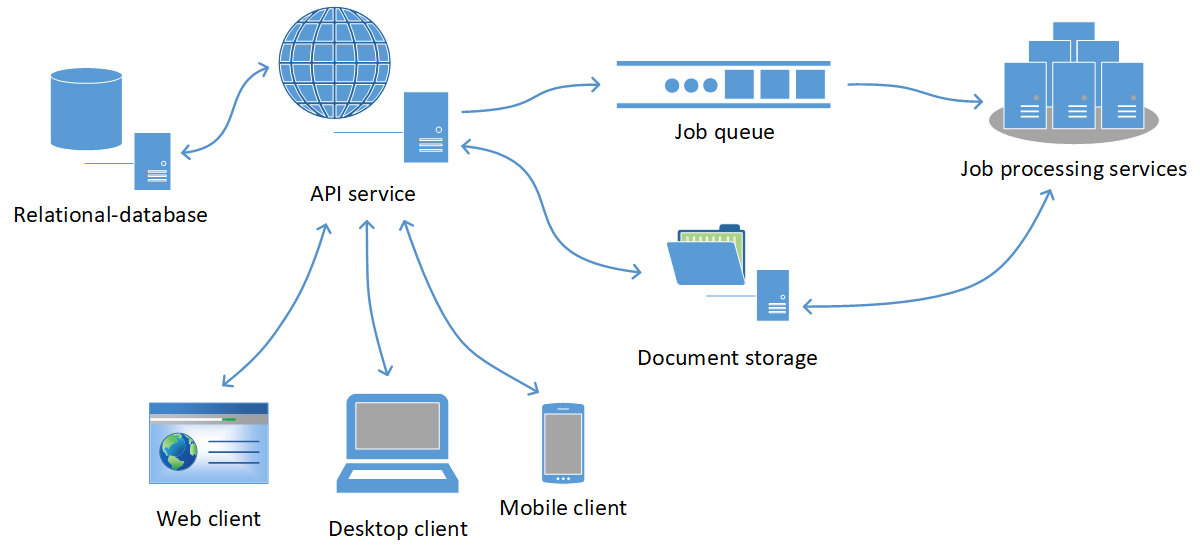
\includegraphics[width=\textwidth]{figures/chapter-data-management/FEA-architecture}
    \decoRule
    \caption{FEA system architecture.}
    \label{fig:FEA-architecture}
\end{figure}

The system contains two types of data storage. The relational-database type of storage is intended to store basic project-related data such as description of simulations, links to the simulation resources, information about the owner and other colaborating users, etc. The input to FEA -- geometrical model, attribute assignments, and analysis parameters -- can also be stored in a relational database, eventhough, storing this complex type of information in the SQL database is questionable and has its drawbacks.

The second type of storage is the blob storage used to hold temporary files being the input or the output of particular components, especially the mesh generator and the FEM solver. The system is designed to be independent of the solver and mesh generator components, therefore this intermediate step of converting the input to proprietary file format that the components understand is necessary. In the future, it is possible to expect a gradual transition from the file-based approach to the direct connection to the database and query the input model directly. Also, the output of the calculation could be saved directly in the proposed format to represent the results in post-process-ready form.

Workflow diagram in Figure \ref{fig:FEA-workflow} helps to visualize the sequence of FEA steps and the transfer of data between the service components. The vertical bars denote computational intensive tasks performed by the service components. The client side in the diagram represents the presentation layer of the FEA system that the user directly interacts with. In the presentation layer, also called \textit{frontend}, there is spent the vast majority of time by users doing pre- and post-processing of data (which is not depicted in the diagram). The web API service, also called \textit{backend}, is the key component that assigns work to other components. It serves as an controller for a running analysis and as an interface between the data stored in databases and the client applications.

\begin{figure}[H]
    \centering
    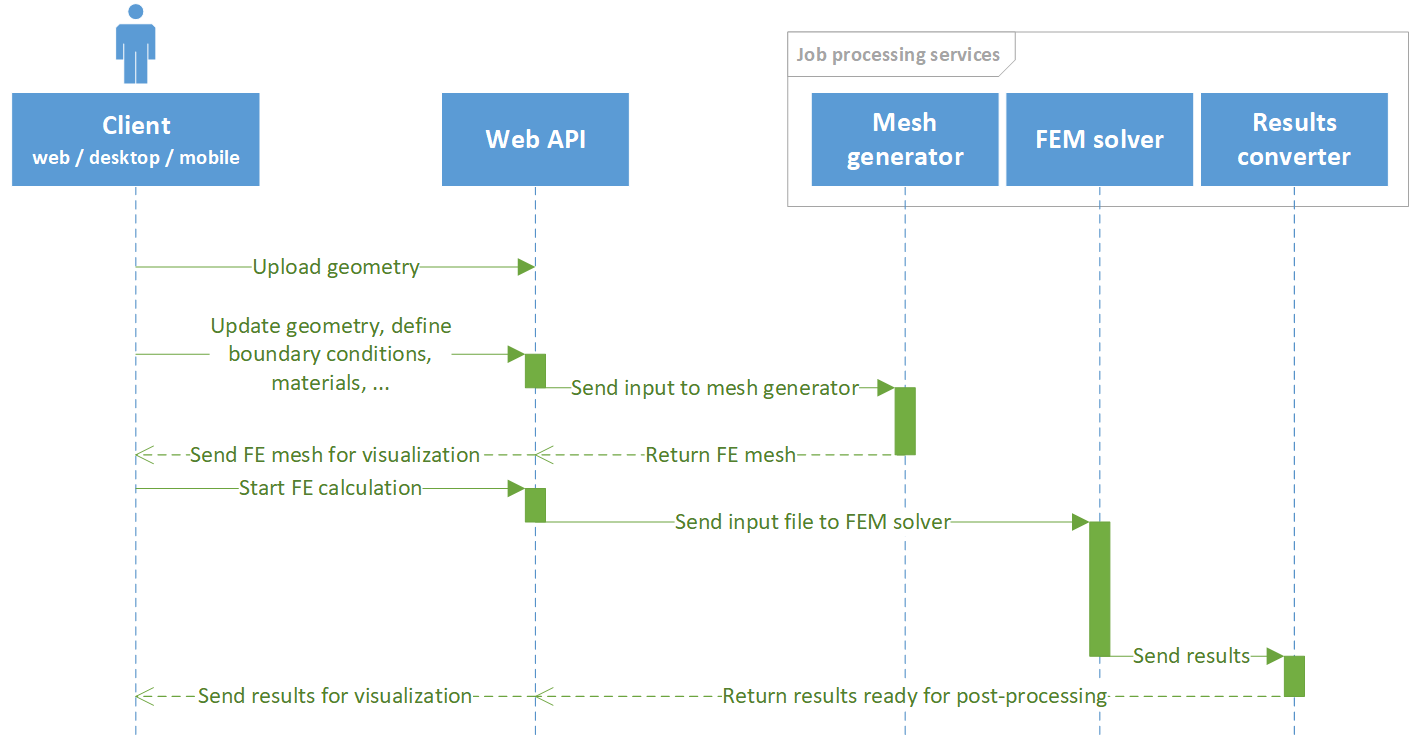
\includegraphics[width=\textwidth]{figures/chapter-data-management/FEA-workflow}
    \decoRule
    \caption{FEA system workflow.}
    \label{fig:FEA-workflow}
\end{figure}

The prototype implementation of the data management system follows the schema and the workflow depicted in Figures \ref{fig:FEA-architecture} and \ref{fig:FEA-workflow}. The difference is that the pre-processing phase is currently excluded. The focus of the work presented in the thesis is primarily on the post-processing features and the representation of results. Therefore, the results from the existing FEM solver are uploaded into the system and the system converts them to the internal representation suitable for post-processing. To test the prototype implementation of the data management system, two client applications are created. The first is the feature-rich desktop post-processor with the support for Linux and Windows operating systems. The second is the simple web application that provides basic control over an analysis and basic post-processing capabilities. Its purpose is mainly to demonstrate the benefits of proposed format for storage of results when post-processing complex FEA. Its web-based implementation allows for truly cross-platform experience without the need for installation and it allows to access the analysis data even from low-end mobile devices.


\section{Storage format for results}
\label{sec:storage-format}

The project-based data model with the representation of simulation results is depicted in Figure \ref{fig:FEA-db-schema-results} as ER diagram.

\begin{figure}[H]
    \centering
    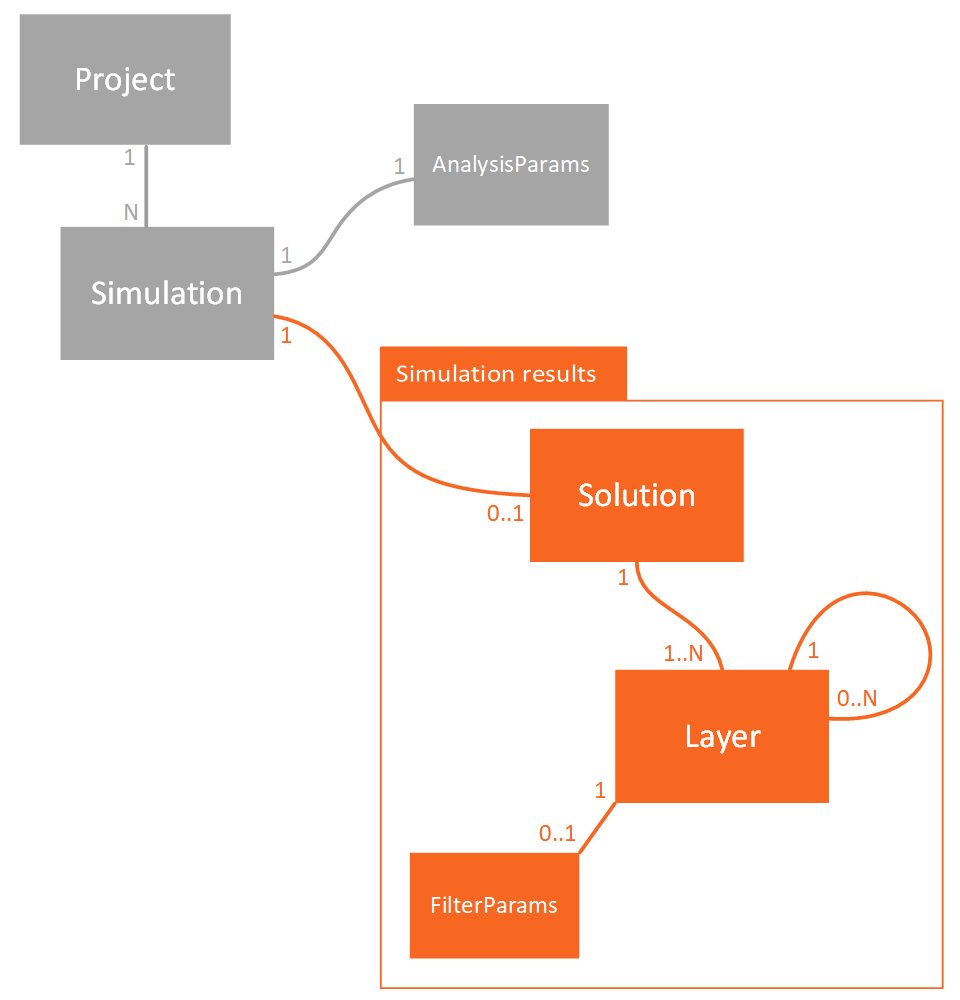
\includegraphics[width=0.8\textwidth]{figures/chapter-data-management/FEA-database-schema-only-results}
    \decoRule
    \caption[Database schema for FEA with results representation only.]{Database schema for FEA with results representation only (without the input model).}
    \label{fig:FEA-db-schema-results}
\end{figure}

The simulation results are represented by the Solution entity, which holds a structure consisting of the results from the FEM solver that are converted to the form suitable for post-processing. The structure has the form of a tree. A node of the tree is represented by the Layer entity. A layer is an association of a mesh and corresponding result fields and other attributes. The use of a tree structure allows to preserve the relations between the parent layers and the layers that are derived from them. The mesh that is referenced by a layer need not be the same as the mesh used as the input mesh to the FEM solver. It could be modified by the solver during the calculation, e.g., due to the use of adaptive finite element techniques. Also, the resulting mesh can be further modified to facilitate the post-processor implementation, e.g., a deformed mesh that helps to visualize the displacement results can be generated, or a number of cross-sections can be created at uniform intervals to provide a look on results inside the mesh. Generally, multiple views on the results can be prepared in advance before the user even starts to investigate the results.

The concept of layer is not new. It is used in existing implementations of the post-pro\-ces\-sors in FEA software packages (often named \textit{filter} instead of layer), to represent a view on the results. However, the layers (visual filters) are usually generated on demand by specific user request and they are not kept in a persistent storage. The proposed storage format for results is built on top of the layer tree structure directly, which allows the layers to be accessed later on, even on a different device, or shared by multiple users working on the same project.


\subsection{Format specification}

The key part of the format is the solution document that holds the information about the layer tree structure. An example of the solution document is given in Listing \ref{lst:solution.json}. In case of remote storage, the solution document is stored in a relational database as part of the project-based data representation shown in Figure \ref{fig:FEA-db-schema-results}, while the rest of documents is stored in a blob storage as group of JSON documents. In case of local storage, all documents, including the solution document, are stored in a folder as JSON files in local file system on a personal computer on which the results are post-processed.

\begin{lstlisting}[style=json,caption=Example of solution.json document.,label=lst:solution.json]
    {
        "Id": 42,
        "ProjectName": "Shear beam 3D",
        "Location": "https://fea-cloud-service.net/postprocess/42",
        "Layers": [
          {
            "Id": "5b585758-9f64-4790-a765-64709951931a",
            "Name": "master",
            "FilterType": null,
            "Children": [
              {
                "Id": "09dfdc8c-a75b-48e1-b319-a9624312a5a5",
                "Name": "deformation (scale: 0.6)",
                "FilterType": "Deformation",
                "Children": [
                  {
                    "Id": "ee52969e-f862-4daf-85b9-5a8224197669",
                    "Name": "slice (offset: -0.1569261)",
                    "FilterType": "Slice"
                  }
                ]
              },
              {
                "Id": "96ca950c-0767-4439-b57a-35384ea351a7",
                "Name": "isosurface DISPLACEMENTS/X(1) = -0.0001",
                "FilterType": "IsoSurface"
              }
            ]
          }
        ]
    }
    \end{lstlisting}

\vspace{5mm}

Data in each layer are stored in four types of documents. All documents are identified by the layer id, which is a GUID (Globally Unique IDentifier), and by its index within the layer (except Summary document that does not need an index as it exist in one instance per layer).

\begin{itemize}

    \item \textbf{Summary document} contains all the descriptive information about a layer. It has the layer id, name, and the the id of the parent layer. It also holds the collection of mesh, result, and attribute descriptors that reference the other documents related to the layer. An example of a summary document in JSON format is presented in Listing \ref{lst:summary.json}.

    \pagebreak

    \begin{lstlisting}[style=json,caption=Example of summary.json document.,label=lst:summary.json]
    {
        "Id": "5b585758-9f64-4790-a765-64709951931a",
        "Name": "master",
        "ParentId": null,
        "Filter": null,
        "Meshes": [
          {
            "Index": 1,
            "TimeSteps": [1.0, 2.0, 3.0, 4.0, 5.0, 6.0],
            "Attributes": [
              {
                "Index": 1,
                "FieldName": "ElementProperty",
                "Location": "Cells"
              }
            ]
          }
        ],
        "Fields": {
          "DISPLACEMENTS": {
            "Components": {
              "X(1)": {
                "TimeSteps": {
                  "1": { "MeshIndex": 1, "DataIndex": 4 },
                  "2": { "MeshIndex": 1, "DataIndex": 4 },
                  "3": { "MeshIndex": 1, "DataIndex": 4 },
                  "4": { "MeshIndex": 1, "DataIndex": 4 },
                  "5": { "MeshIndex": 1, "DataIndex": 4 },
                  "6": { "MeshIndex": 1, "DataIndex": 4 }
                }
              },
              "X(2)": { ... },
              "X(3)": { ... }
            }
          },
          "CRACK_WIDTH": { ... },
          "EXTERNAL_FORCES": { ... },
          "STRAIN": { ... },
          "STRESS": { ... }
        }
    }
    \end{lstlisting}
    
    \item \textbf{Mesh document} contains the geometric representation of a finite element mesh. An example of a mesh document in JSON format is presented in Listing \ref{lst:mesh.json}.
    
    \begin{lstlisting}[style=json,caption=Example of mesh.json document.,label=lst:mesh.json]
        {
            "LayerId": "5b585758-9f64-4790-a765-64709951931a",
            "Index": 1,
            "NumberOfPoints": 434,
            "NumberOfCells": 324,
            "Center": [0.6375, 0.095, 0.16],
            "Radius": 0.6719607,
            "PointCoordinates": "//9/MwAAADIK16M+//9/MwAAADJvEoM+gDSjPQAAADIK16M+//9/M1yPwj0K16M+gDSjPQAAAD...",
            "CellConnectivity": "SwAAADgAAAA0AAAASQAAAD4AAAArAAAAKAAAADwAAAA+AAAAKwAAACgAAAA8AAAAOQAAACUAAA...",
            "CellTypes": "DAwMDAwMDAwMDAwMDAwMDAwMDAwMDAwMDAwMDAwMDAwMDAwMDAwMDAwMDAwMDAwMDAwMDAwMDAwMDAwMD..."
        }
    \end{lstlisting}

    \item \textbf{Attribute document} serves as a container for additional information assigned to mesh entities, e.g., material id of each finite element. An example of an attribute document in JSON format is presented in Listing \ref{lst:attribute.json}.

    \begin{lstlisting}[style=json,caption=Example of attribute.json document.,label=lst:attribute.json]
        {
            "LayerId": "5b585758-9f64-4790-a765-64709951931a",
            "Index": 1,
            "MeshIndex": 1,
            "FieldName": "ElementProperty",
            "Location": "Cells",
            "Compression": null,
            "Encoding": {
              "DataType": "Int32",
              "OriginalLength": 324,
              "Offset": 160,
              "Length": 164,
              "DefaultValue": "18"
            },
            "Data": "EwAAABMAAAATAAAAEwAAABMAAAATAAAAEwAAABMAAAATAAAAEwAAABMAAAATAAAAEwAAABMAAAATAAAAEwAAAB..."
        }
    \end{lstlisting}

    \item \textbf{Result document} is the document that contains the result fields from FEM. An example of a result document in JSON format is presented in Listing \ref{lst:result.json}. Result document is usually the most memory-consuming component of the storage format and it is therefore designed to support compression of data to reduce its size. The compressed data are converted to text using a binary-to-text encoding method and stored as the value of \code{Data} property.

    There are also many options to partition the data into smaller groups. The largest granularity is achieved when the data corresponding to a single time step is stored in a single document, which allows for the lowest latency when transfering the document from the storage to the post-processor, in particular when the data are stored on a remote machine. On the other hand, the better reduction of overall size can be achieved when the data for all time steps of a field component are stored together in one document, which usually leads to better compression ratio as the compression method can find more redundancies in the data.

    \begin{lstlisting}[style=json,caption=Example of result.json document.,label=lst:result.json]
        {
            "LayerId": "5b585758-9f64-4790-a765-64709951931a",
            "Index": 4,
            "MeshIndex": 1,
            "FieldName": "DISPLACEMENTS",
            "ComponentName": "X(1)",
            "TimeSteps": [1.0, 2.0, 3.0, 4.0, 5.0, 6.0],
            "Location": "Points",
            "Compression": {
              "Method": "SVD",
              "Rows": 6,
              "Columns": 434,
              "Rank": 3
            },
            "Encoding": {
              "DataType": "Float64",
              "OriginalLength": 2640,
              "Offset": 0,
              "Length": 2640
            },
            "Data": "47HYqWHLML9OLoc9P8tAv5nfIqKPa1S/BoMRvASgbL+E47yyIMJ5v47IymmBdYK/ZcAwsn55IL+uuEUHN3swv1..."
        }
        \end{lstlisting}

\end{itemize}

% TODO: remove this paragraph?
\vspace{5mm}

At first glance the format seams to be overcomplicated. The data are scattered throughout a large number of documents. There are various types of documents with different schema, some information is duplicated, etc. However, the format is carefully designed to allow efficient and simple implementation of a post-processor while enabling the use of compression to significantly reduce the storage size of the results if needed. A post-processor should be able to easily decode the data and display it immediately, without the need for additional transformation, sorting, or caching. E.g., there is one-to-one mapping of the data in a result document to a mesh to be able to use the decoded data array directly as an OpenGL buffer in the graphics card. Also, the fact that the data are stored in a small structured documents of a known schema enables to index the data by a database management system and also to create efficient queries over the data. As a side effect of the data fragmentation, the resulting latency is being very low, i.e., the delay between the user request and the data being rendered on a screen is small (which allows real-time creation of animations).

\chapter{SVD used for compression of FEA results}

Singular Value Decomposition (SVD) is a well known factorization method that provides rich information about matrix systems \cite{Baker2005, Kalman1996, Golub1996, Duintjer2012}. One of its many applications is image compression where it can significantly reduce size of data representing image while preserving quality of image appearance. Considering the fact that the results from FEM analyses can be viewed as a series of arbitrary rectangular matrices, the implementation of compression algorithm based on SVD is straightforward as SVD can be applied to any rectangular matrix. The compression method based on SVD is the key part of the storage format proposed in the thesis.


\section{Definition}

Singular value decomposition is based on a theorem from linear algebra which says that a rectangular matrix $\mtrx{A} \in \mathbb{R}^{m \times n}$ can be decomposed into the product of three matrices - an orthogonal matrix $\mtrx{U} \in \mathbb{R}^{m \times m}$, a diagonal
matrix $\mtrx{S} \in \mathbb{R}^{m \times n}$, and the transpose of an orthogonal matrix $\mtrx{V} \in \mathbb{R}^{n \times n}$:

\begin{equation}
\mtrx{A} = \mtrx{U} \mtrx{S} \mtrx{V}^\mathsf{T},
\label{eq:svd-def}
\end{equation}

\noindent
where $\mtrx{U^\mathsf{T}U} = \mtrx{I}$, $\mtrx{V^\mathsf{T}V} = \mtrx{I}$. The columns of $\mtrx{U}$ are orthonormal eigenvectors of $\mtrx{AA^\mathsf{T}}$, which are called the left singular vectors. The columns of $\mtrx{V}$ are orthonormal eigenvectors of $\mtrx{A^\mathsf{T}A}$ called the right singular vectors. $\mtrx{S}$ (sometimes referred to as $\mtrx{\Sigma}$) is a diagonal matrix containing singular values in descending order, which are at the same time the nonzero square roots of the eigenvalues of $\mtrx{AA^\mathsf{T}}$ and $\mtrx{A^\mathsf{T}A}$.

SVD can be seen as a method for transforming correlated variables into a set of uncorrelated ones. At the same time, SVD is a method for ordering the dimensions based on variation and identifying the dimension with the largest variation. Once this dimension is identified, it is possible to find the best approximation of the original data points using fewer dimensions. Hence, SVD can be seen as a method for data reduction/compression.

From the definition of SVD in (\ref{eq:svd-def}) and from the properties of SVD, the fact follows that a matrix can be represented in the form of its SVD components as a sum of $k$ rank-1 matrices

\begin{equation}
\mtrx{A}=\sum_{i=1}^{k} s_{i}\mathbf{u}_{i}\mathbf{v}_{i}^{\mathsf{T}},
\label{eq:svd-expansion}
\end{equation}

\noindent
where $s_i$ is the $i$-th singular value of matrix $\mtrx{A}$, $\mathbf{u}_i$ and $\mathbf{v}_i$ are corresponding singular vectors of matrix $\mtrx{A}$, and $k = \mathrm{min}(m, n)$. Considering the fact that singular values are ordered $s_{1} \geq s_{2} \geq s_{3} \geq ... \geq s_{k}$, the above formula implies that the first term of the sum would have the highest contribution and the last term would have the lowest contribution to matrix~$\mtrx{A}$. Therefore, if we take only first $r$ members of the above summation we get an \textbf{low-rank approximation matrix}

\begin{equation}
\mtrx{A'}=\sum_{i=1}^{r} s_{i}\mathbf{u}_{i}\mathbf{v}_{i}^{\mathsf{T}}.
\label{eq:svd-approx-expansion}
\end{equation}


Quality of approximation depends on the magnitude of the singular values omitted from the approximation formula, namely $s_{r+1} ...  s_{k}$. The compression algorithm is based on an assumption that the first singular value is order-of-magnitude higher than singular values at the end of the decomposition sequence. In special cases, when $r=k$, or $s_{i}=0$ for all $i > r$, the omitted singular values do not contribute to the sum and the compression is therefore lossless. In other cases, approximation error has to be calculated and taken into account to avoid loss of important details in data.

The main goal of the compression algorithm is to find a compromise between low approximation error and high compression ratio $c$ which is calculated using the formula

\begin{equation}
c=\frac{r(m+n+1)}{m n},
\label{eq:cr-def}
\end{equation}

\noindent
where $m$ is the number of rows and $n$ is the number of columns of matrix $\mtrx{A}$. Explanation of the compression ratio formula is best done using Figure~\ref{fig:lowrank_svd}. Light color represents the part of matrix decomposition that is to be stored in the output file as a low-rank approximation of the input.

\begin{figure}[H]
\centering
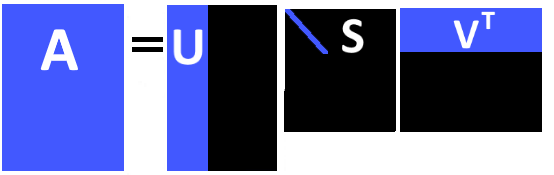
\includegraphics[width=0.7\textwidth]{figures/chapter-SVD/low_rank_decomposition_diagram}
\decoRule
\caption[Singular value decomposition illustration.]{Decomposition of input matrix $\mtrx{A}$ into diagonal matrix of singular values $\mtrx{S}$ and matrices of left and right singular vectors. Light color illustrates low-rank approximation.}
\label{fig:lowrank_svd}
\end{figure}


Compression based on a low-rank approximation matrix is a lossy compression method. To quantify the error, the Normalized root-mean-square deviation ($\mathit{NRMSD}$) is used. It is defined as

\begin{equation}
\mathit{NRMSD} = \frac{\mathit{RMSD}}{X_{max}-X_{min}}=\frac{\sqrt{\mathit{MSE}}}{X_{max}-X_{min}},
\label{eq:nrmsd-def}
\end{equation}

\noindent
where $X_{min}$ and $X_{max}$ are elements of input matrix $\mtrx{A}$ with minimum and maximum value, respectively. This error metric is able to measure and compare errors in datasets with different scales. Therefore, it is the main parameter that is used to control the quality of compression in the proposed compression algorithm.

\section{Implementation}

Results from the finite element method are scalar, vector or tensor fields represented by discrete values calculated in nodes of the mesh or in integration points on finite elements. In order to compress data, an auxiliary matrix~$\mtrx{A}$ has to be assembled from the results. The number of rows of the matrix~$\mtrx{A}$ is equal to the number of incremental or time steps while the number of columns is equal to the number of points in which the results are stored. Such auxiliary matrix is assembled for each scalar field and for each component of the vector and tensor fields. It means, three matrices corresponding to the displacement in the $x$, $y$, and $z$ directions are assembled for the vector of displacements in three-dimensional problems.

There are two main reasons to store particular results in separate matrices. First, the size of matrices is smaller than the size of a matrix which contains all results and therefore SVD will be performed faster. Second, the magnitudes of particular fields are very different (the stress tensor components are several order of magnitude larger than the components of the displacement vector) and the data compression algorithm would suppress the fields with small magnitudes. Once the matrix $\mtrx{A}$ is assembled for each field, the compression algorithm can be applied on it. It is purely algebraic procedure and no information about geometry of the mesh is needed.

Let us assume that the matrix is not empty and it is full rank. Then it follows from the formula (\ref{eq:cr-def}) that if $r$ is equal to the rank of matrix $\mtrx{A}$, the compression ratio is always higher than one. In other words the memory consumption of stored decomposition is bigger than the size of the original matrix. To make the compression algorithm applicable, the parameter $r$ must satisfy the condition

\begin{equation}
r<\frac{m n}{m+n+1}.
\label{eq:r-ineq}
\end{equation}

\noindent
Considering the usual shape of matrix containing FEM results, this inequality is easily satisfiable even for the $r$ being close to the rank of the original matrix as in the typical case the number of nodes or integration points is much higher than the number of analysis steps and therefore $m \ll n$.


\section{Randomized SVD}

There are many algorithms with different approaches to compute singular value decompositions. One approach is based on diagonalization of the matrix which essentially yields the whole decomposition at the same time. The other approach is the use of an iterative algorithm that yields one or several singular values at a time and can be stopped after desired number of singular values and vectors has been computed. Although these algorithms have proven to work very well for relatively small matrices, they are not well suited for using with large data sets. The exact SVD of a $m \times n$ matrix has computational complexity $\mathrm{O}(\mathrm{min}(mn^2, m^2n))$ using the ``big-O'' notation. When applied on large data sets it tends to be very time-consuming. Also, the modern hardware architectures use caches to optimize reading of consecutive memory blocks. As these algorithms often need random access to the memory where the input matrix is stored, it can increase communication between different levels in memory hierarchy, which causes higher latency when accessing data. From a numerical linear algebra perspective, an additional problem resulting from increasing matrix sizes is that noise in the data, and propagation of rounding errors, become increasingly problematic.

In \cite{Candes2011, Woolfe2008, Martinsson2011, Szlam2014}, there are described randomized methods for constructing approximate matrix factorizations which offer significant speedups over classical methods. The particular implementation of the randomized decomposition is based on the algorithm described in \cite{Halko2011}. The authors proposed an algorithm for efficient computation of low-rank approximation to a given matrix. The method uses random sampling to identify a subspace that captures most of the action of a matrix. The input matrix is compressed to this subspace, and deterministic manipulations are then used to obtain the desired low-rank factorization. For a matrix that is too large to fit in fast memory, the randomized techniques require only a constant number of passes over the data, as opposed to $\mathrm{O}(k)$ passes for classical algorithms.
\chapter{Results}

\section{SVD compression method results}

First example is an analysis of aging of nuclear power plant's containment made from prestressed concrete. The finite element mesh used in this analysis is in Figure \ref{fig:temelin:mesh}. More details about the analysis can be found in \cite{Kruis2012} and \cite{Koudelka2009}. This analysis includes high number of analysis time steps (thousands) with very little differences between them. There is therefore potential for compression to be very effective (compression ratio to be very low) as proven in Figure \ref{fig:temelin:NRMSD} that examines the impact of changes in the compression ratio to the mean error of approximation.

\begin{figure}[H]
\centering
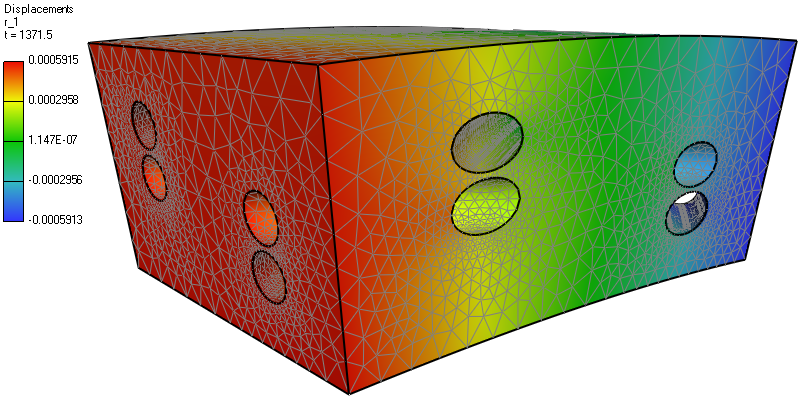
\includegraphics[width=\textwidth]{figures/chapter-SVD/temelin_screenshot}
\decoRule
\caption[Results visualization: reactor containment 3D.]{Segment of reactor containment analyzed. Results visualization (displacement field, x component).}
\label{fig:temelin:mesh}
\end{figure}

\begin{figure}[H]
\centering
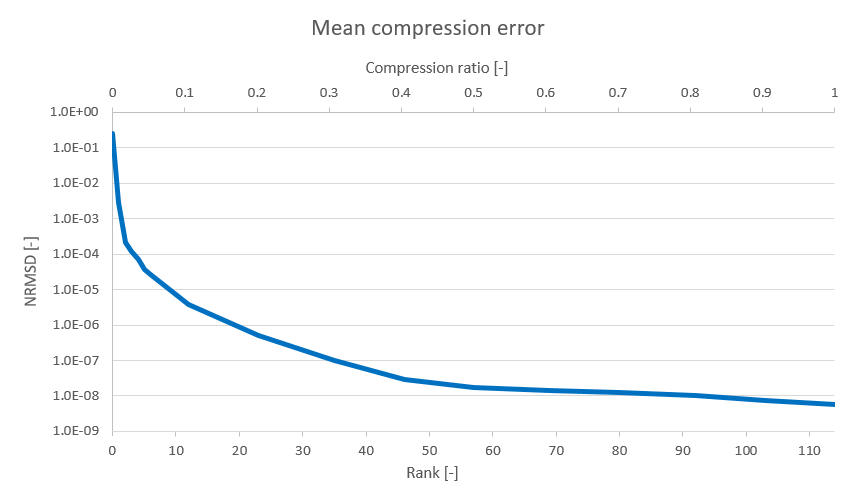
\includegraphics[width=\textwidth]{figures/chapter-SVD/temelin_NRMSD}
\decoRule
\caption[Dependence of NRMSD on compression ratio and rank (reactor containment 3D).]{Dependence of $\mathit{NRMSD}$ on $c$ and $r$ for reactor containment analysis results.} % ...$c$ (and $r$)...
\label{fig:temelin:NRMSD}
\end{figure}

% Execution times
Besides the error also the execution speed of compression algorithm was measured. In Figure \ref{fig:temelin:ExeTime}, there is a comparison of execution times for standard versus randomized SVD compression algorithms. Interestingly, execution time of standard SVD is independent of target rank whereas execution time of randomized SVD decreases linearly with decreasing target rank. If the rank is known ahead, the fact can be taken advantage of.

\begin{figure}[H]
\centering
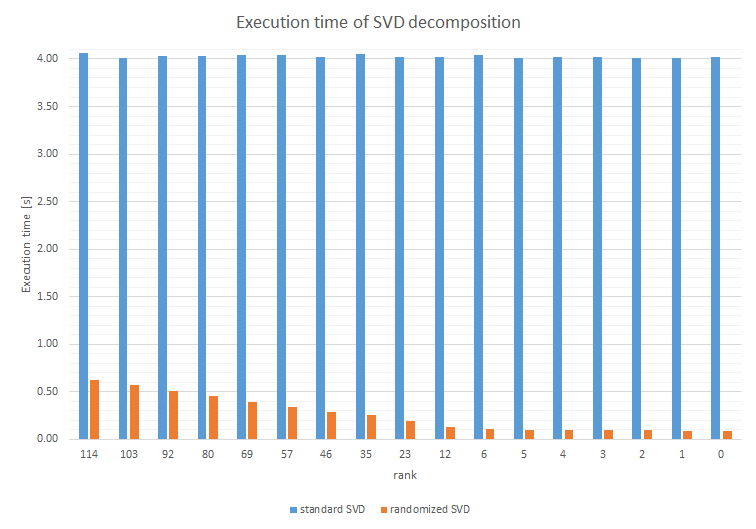
\includegraphics[width=\textwidth]{figures/chapter-SVD/temelin_ExecutionTime}
\decoRule
\caption[Execution time of standard and randomized SVD decompositions.]{Variation of execution time of standard and randomized SVD decompositions calculated for reactor containment analysis results.}
\label{fig:temelin:ExeTime}
\end{figure}

\section{Post-processor implementation results}

% Post-processors screenshots and description

This section contains screenshots and performance evaluation of both the desktop post-processor and the web post-processor. In Figure \ref{fig:desktop-postprocessor-remote-solutions}, there is a screenshot of the desktop post-processor that demonstrates the ability to connect to the remote web API and retrieve the list of solutions stored in the database.

\begin{figure}[H]
    \centering
    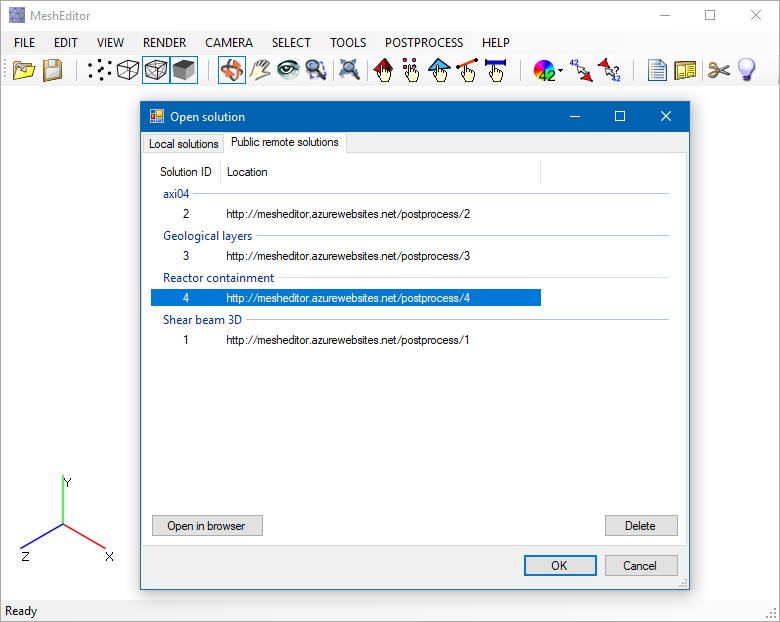
\includegraphics[width=\textwidth]{figures/chapter-data-management/desktop-postprocessor-remote-solutions}
    \decoRule
    \caption[Desktop post-processor screenshot. List of remote solutions.]{Desktop post-processor screenshot. Demonstration of connection to the web API (listing of remote solutions).}
    \label{fig:desktop-postprocessor-remote-solutions}
\end{figure}

Figure \ref{fig:desktop-postprocessor-master} shows the visualization of the master layer of the selected solution in the desktop post-processor window. The left panel contains the layer tree view that allows to choose the layers to show in the main window. There are also the options to visualize components of scalar, vector, or tensor data using the color scale on the mesh surface. Vector fields can be also visualized using arrows in the data locations pointing in the direction corresponding to the vector field. The top panel contains the tools for manipulation with the mesh, changing the camera view, selecting mesh entities, and assigning attributes to them.

\begin{figure}[H]
    \centering
    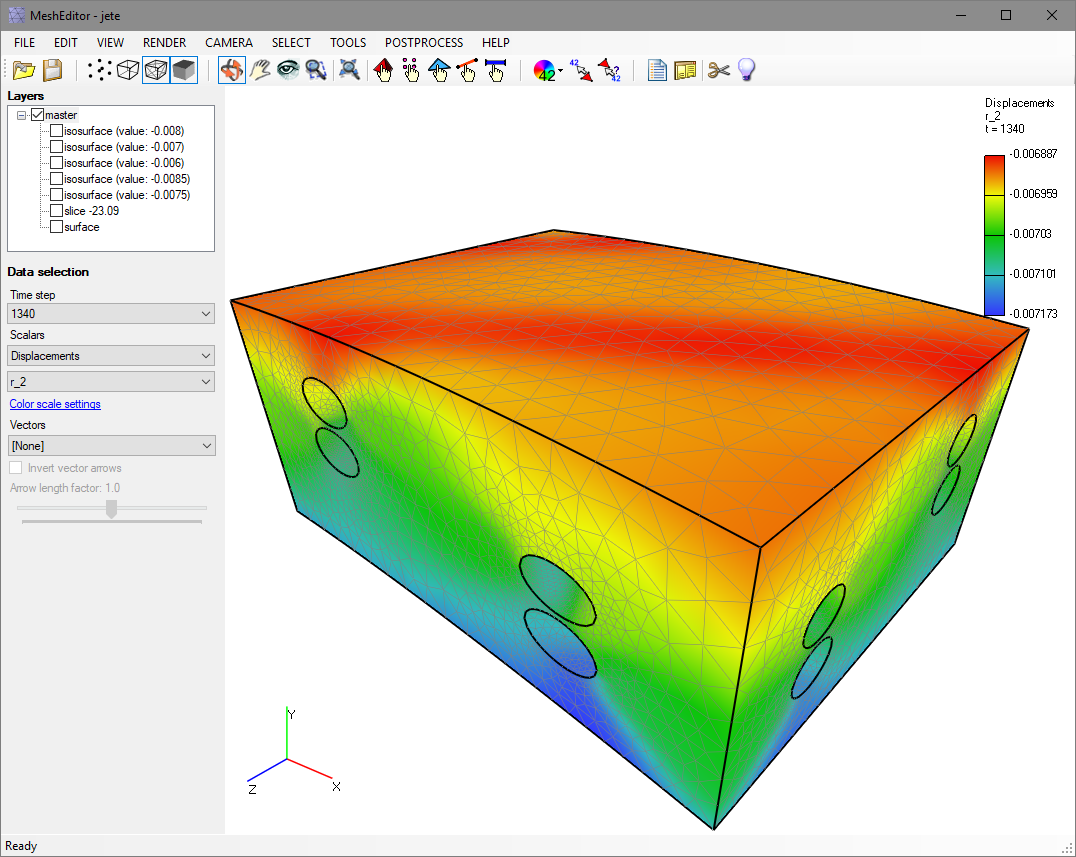
\includegraphics[width=\textwidth]{figures/chapter-data-management/desktop-postprocessor-master}
    \decoRule
    \caption{Desktop post-processor screenshot. Visualization of a master layer.}
    \label{fig:desktop-postprocessor-master}
\end{figure}

The post-processor also provides the user interface for definition of the parameters of a visual filter that the user wants to be applied on the selected layer. The parameters are sent as a part of the filter command that is sent to the FEM format converter component that generates the new layer. The layer tree is then updated and the new layer is displayed. The examples of slice and iso-surface layers are shown in Figure \ref{fig:desktop-postprocessor-slice} and Figure \ref{fig:desktop-postprocessor-isosurface}, respectively.

\begin{figure}[H]
    \centering
    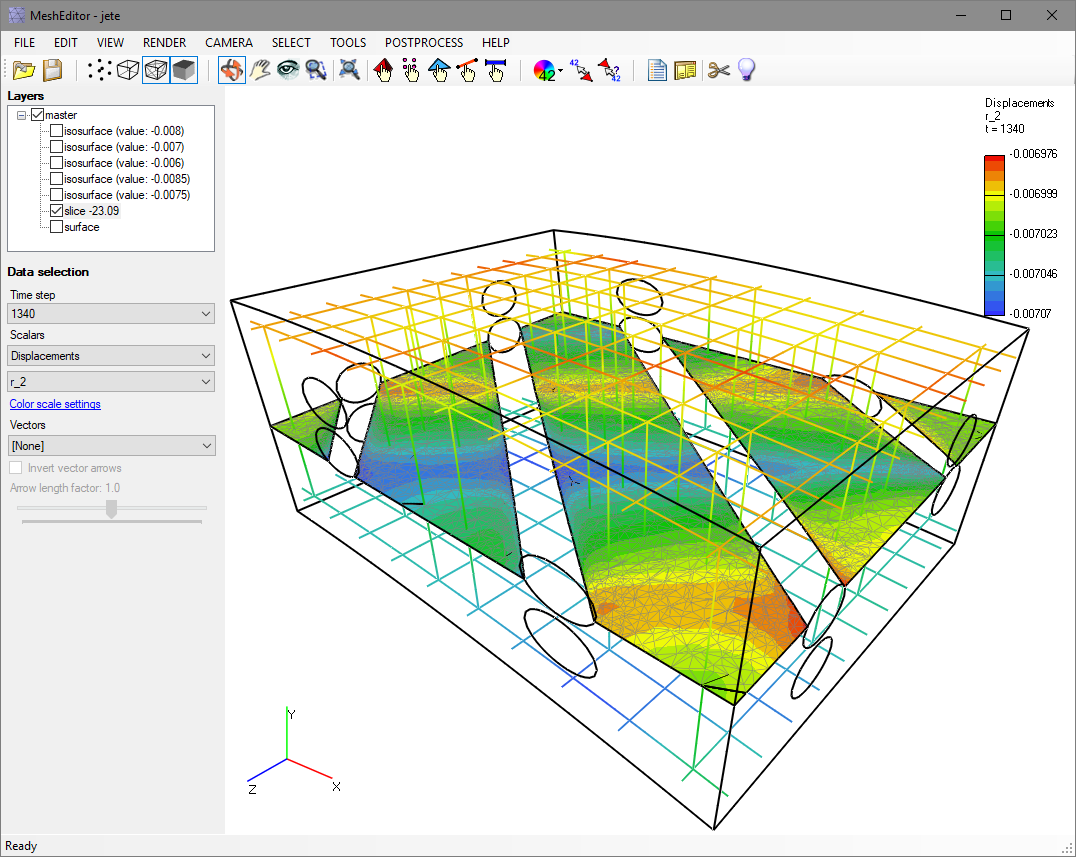
\includegraphics[width=0.85\textwidth]{figures/chapter-data-management/desktop-postprocessor-slice}
    \decoRule
    \caption{Desktop post-processor screenshot. Visualization of a slice layer.}
    \label{fig:desktop-postprocessor-slice}
\end{figure}

\begin{figure}[H]
    \centering
    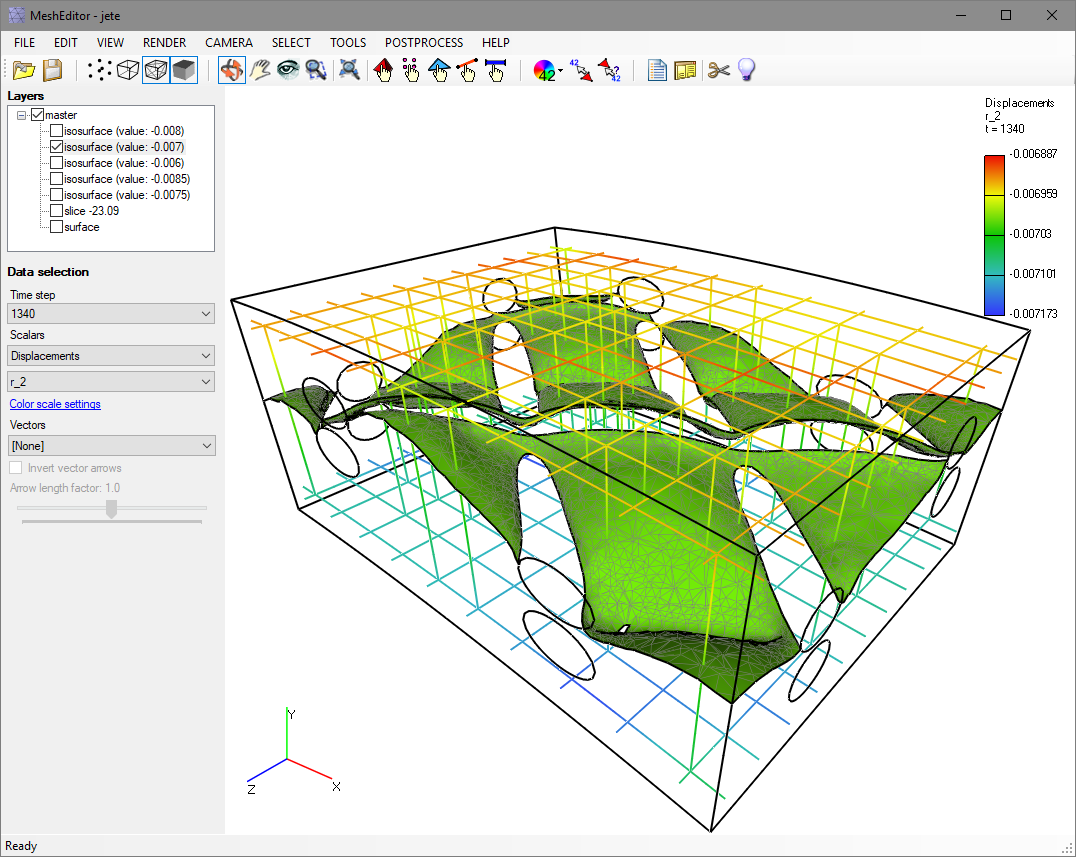
\includegraphics[width=0.85\textwidth]{figures/chapter-data-management/desktop-postprocessor-isosurface}
    \decoRule
    \caption{Desktop post-processor screenshot. Visualization of a iso-surface layer.}
    \label{fig:desktop-postprocessor-isosurface}
\end{figure}


\begin{figure}[H]
    \centering
    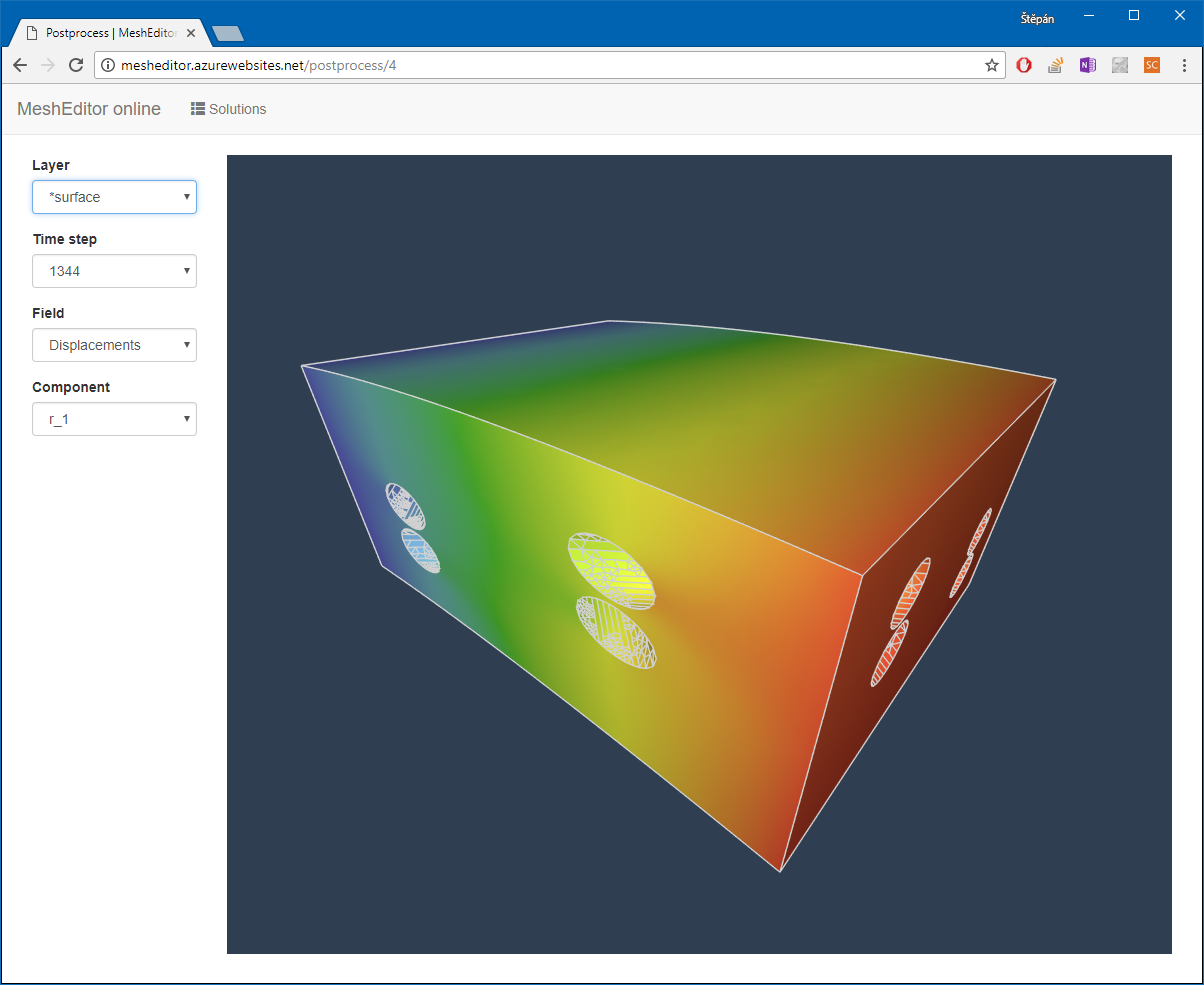
\includegraphics[width=0.75\textwidth]{figures/chapter-data-management/web-postprocessor-surface}
    \decoRule
    \caption{Web post-processor screenshot. Visualization of a surface layer.}
    \label{fig:web-postprocessor-surface}
\end{figure}

\begin{figure}[H]
    \centering
    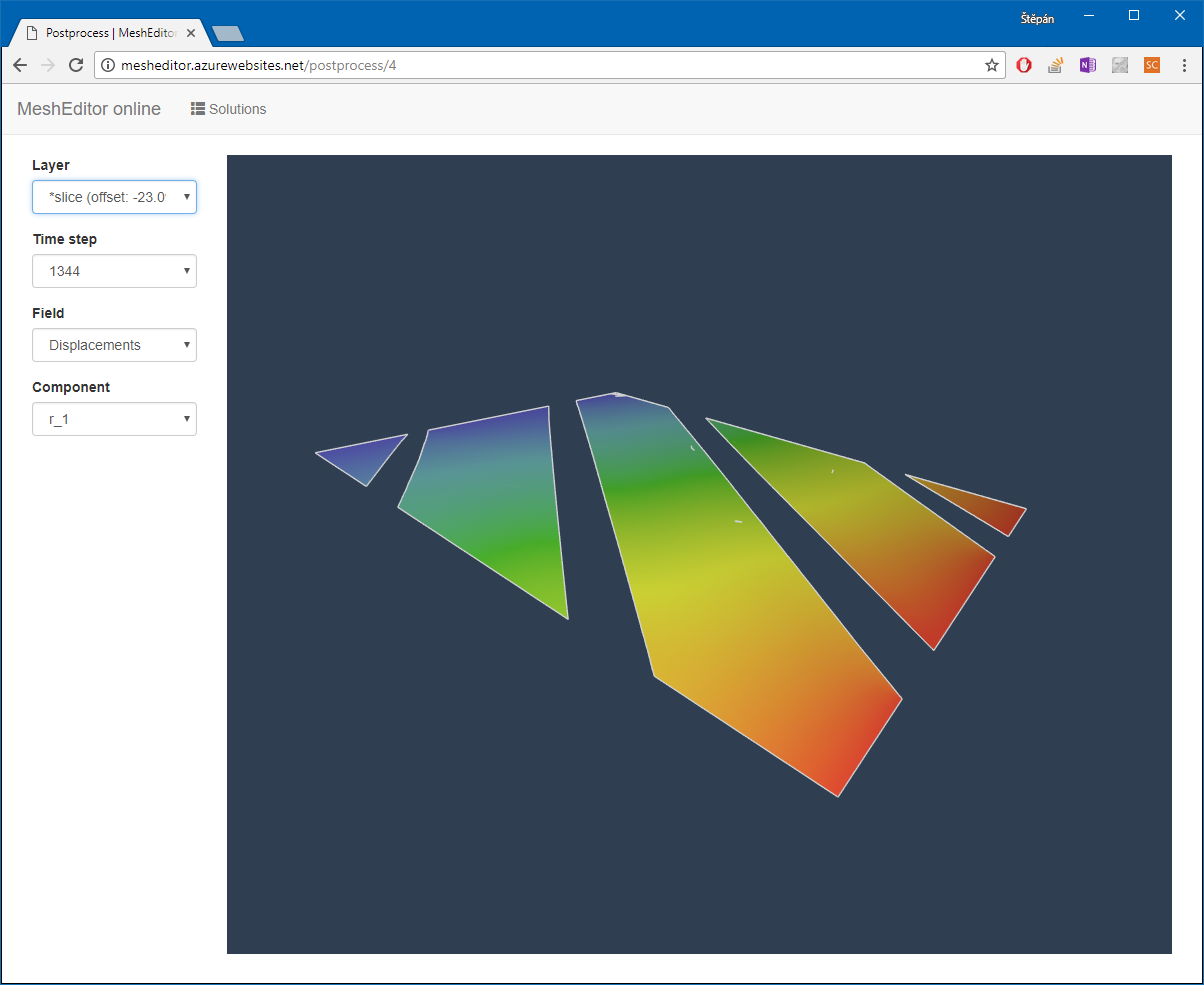
\includegraphics[width=0.75\textwidth]{figures/chapter-data-management/web-postprocessor-slice}
    \decoRule
    \caption{Web post-processor screenshot. Visualization of a slice layer.}
    \label{fig:web-postprocessor-slice}
\end{figure}

Figure \ref{fig:web-postprocessor-surface} shows the web post-processor that is connected to the same database as the desktop post-processor. The user interface also allows to select the layer of the current solution and the data component that should be visualized on the mesh surface. Figure \ref{fig:web-postprocessor-slice} contains the visualization of a slice layer.

\begin{figure}[H]
    \centering
    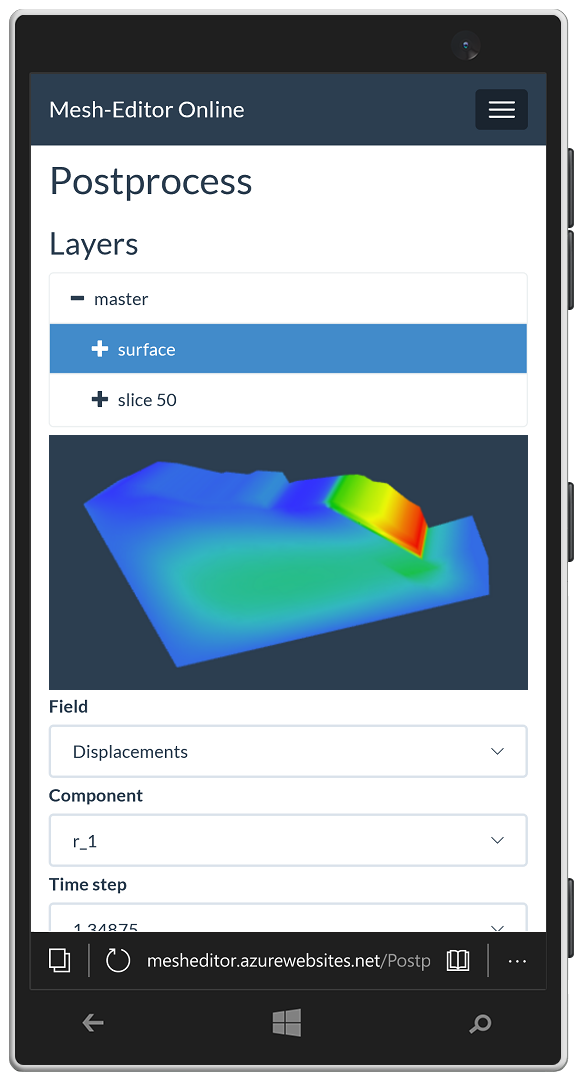
\includegraphics[width=0.35\textwidth]{figures/chapter-data-management/web-postprocessor-mobile}
    \decoRule
    \caption{Web post-processor screenshot taken on a mobile device.}
    \label{fig:web-postprocessor-mobile}
\end{figure}

Figure \ref{fig:web-postprocessor-mobile} demonstrates the fact that the web post-processor is fully capable of running on a mobile device with limited CPU and memory resources. The web application is designed to support multiple form factors and can be used comfortably even on a small device with touch screen.

Generation of a new filter layer is offloaded to the server and can took tens of seconds for large solutions. However, it is a one-time operation because the result is stored in a persistent storage. The subsequent requests for documents containing layer data are very fast. For a common mesh having around 300000 elements the web post-processor needs only tens of milliseconds to render layer geometry and selected data component on the mesh surface, even though it downloads all the necessary data from a remote server over the Internet. This speed allows to avoid caching of the data on the client device and helps to keep the memory consumption of the proposed post-processors very low (tens of megabytes for common mesh sizes) compared to traditional post-processors that need to load and process all the results from a file in order to display selected information.

\chapter{Conclusions}

There were three main goals of the thesis as described in Chapter \ref{chapter:aims}. The first goal was to design a new storage format for representation of the results from the finite element method with the support for compression. This goal was fulfilled. Besides the compression, the new storage format allows efficient querying of the data, unlike the standard unstructured file-based formats, which require parsing through the complete set of results to retrieve a specific information. Examples of the proposed format in form of JSON documents are given. Also, the application that can convert the results from the FEM solver to the new storage format was implemented. This converter application further supports generation of visual filters and it is designed to be run either locally on a PC or remotely in a cloud environment.

The second goal of the thesis was to investigate suitable methods for compression of results from FEM and develop a compression algorithm with reasonable performance characteristics and producing approximations with low and predictable error. The compression method based on singular value decomposition satisfies these requirements. The SVD compression method became the integral part of the storage format. The results of its application on real data have been presented. The algorithm is able to compress arbitrary data using low-rank approximation matrices. When the maximum allowed relative error was set to $10^{-5}$, the compression ratio was at most 10\% for all tested results. In many cases, the compression ratio can be even better -- bellow 1\% of the original size. The important property of the compression algorithm is the fact that the approximation error can be set in advance and there is a guarantee that it will not be exceeded. The disadvantage of the SVD-based compression method is the computational complexity. SVD is a very time-consuming operation. However, this operation is performed only once during the conversion of results from FEM solver to the storage format, before the post-processing is started. Also, the randomized version of the decomposition algorithm is much faster and can be used if a slight increase of the approximation error is tolerated. The detailed description of the SVD-based compression method is described in the thesis and also published in \cite{Benes2018}.

The third goal was the implementation of two post-processors that should demonstrate the efficiency of the proposed methods. Both the desktop and the web post-processor were implemented and described in detail. The desktop post-processor is a feature-rich visualization tool that allows to visualize the data in various formats including the new proposed storage format. It is able to create efficient surface representation of an arbitrary finite element mesh and it implements advanced techniques for manipulation with the mesh entities. The detailed description of the implementation is presented in the thesis and published in \cite{Benes2015}. The web-based post-processor is a simple cross-platform application that is able to visualize the simulation results located in a remote storage. As the hard work connected with processing of the results is offloaded to the server, the web application is just a thin client that works even on devices with limited CPU and memory resources.

Besides the presented goals, the thesis also outlines the architecture of the data access system for complex FEA consisting of several independent services. The system is designed as a collaborative framework that can be accessed by users from different client devices. The web post-processor is built on top of this data management system, it directly communicates with the web API service to provide the user with the access to FEA simulations running on a remote server. The database schema for project and simulation related data is given as well as the description of individual services.

% Approximation by polynomials
As a not very suitable method for data reduction is considered the approximation of the FEM results by polynomial functions that is presented in the thesis and published in \cite{Benes2016} and \cite{Benes2016Pollack}. The method was inspired by the multigrid method (and generally other multi-mesh methods, hence the name of the thesis) that was at the beggining of the research work. The multigrid method allows to solve partial differential equations using the hierarchy of domain discretizations. The idea was to connect the FEM solution phase with the post-processing by reusing the mesh hierarchy used by the multigrid method also in the post-processing of the results. Although the presented approximation method is capable of a significant reduction of the data size (down to 2.5\% of the original size), the maximal approximation error can be very high (up to 100\% in extreme cases, e.g., when there are discontinuities or singulatities in the data). The unpredictibility of the error and the high decompression time are the reasons the method is excluded from the implementation of the post-processors in favor of the SVD compression method.


%----------------------------------------------------------------------------------------
%	BIBLIOGRAPHY
%----------------------------------------------------------------------------------------

%\nocite{*} % check for unused references (package refcheck); comment out to filter out unused references

\printbibliography[heading=bibintoc]

%-----------------------------------------------------------------------------
%	List of publications
%-----------------------------------------------------------------------------
%
\chapterwithoutnumber{7}{Publications related to the thesis}


%
%-----------------------------------------------------------------------------
%	COVER
%-----------------------------------------------------------------------------
%

\cleardoublepage % insert blank page after publications

\end{adjustwidth}

\end{document}
